%!TEX TS-program = xelatex
%!TEX encoding = UTF-8 Unicode
\documentclass{article}
\usepackage[provide=*,dutch]{babel}

\usepackage{geometry}
\geometry{a4paper}
\usepackage[utf8]{inputenc}
\usepackage{enumitem}
\usepackage{hyperref}
\usepackage{graphicx}
\usepackage{tcolorbox}
\hyphenation{wacht-tijd}
\hyphenation{wacht-tijden}
\setlength{\textheight}{240truemm}
% For better header handling
\usepackage{fancyhdr}
\pagestyle{fancy}
\fancyhf{}
\lhead{PVA Ingensche Veer}
\chead{IPASS}
\rhead{Vincent van Setten - 1734729}
\rfoot{Pagina \thepage}

% For colored text
\usepackage{xcolor}

\title{IPASS Plan van Aanpak}
\author{Vincent van Setten}

\begin{document}

\begin{titlepage}
    \begin{center}
        \vspace*{.6cm}
        \Huge
        \textbf{Plan van Aanpak }\\
        \vspace{0.2cm}
        \LARGE 
        \textbf{Ingensche Veer} \\
  
        \normalsize
  
  
        \vspace{1cm}
        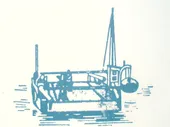
\includegraphics[width=0.7\textwidth]{images/iv.png}
        \vspace{1cm}
        \Large\\
        \textbf{In opdracht van}\\
        \large
        \textbf{University of Applied Sciences Utrecht} \\
        
\includegraphics[width=0.2\textwidth]{images/logouni.jpg}
  
        \vfill
      \end{center}
      \textbf{Datum:} \today \\
      \textbf{Versie:} 1.0 \\
      \textbf{Auteur:} Vincent van Setten \\
      \textbf{Studentnummer:} 1734729 \\
      \textbf{Klas:} V1C\\
  
  \end{titlepage}
  
  % ToC
  \tableofcontents
  \pagebreak 

  \section{Revisie Historie}
  \begin{table}[h]
      \centering
      \begin{tabular}{|c|c|c|p{5cm}|}
          \hline
          \textbf{Versie} & \textbf{Datum} & \textbf{Omschrijving}  \\
          \hline
          1.0  & 19-05-2024 & Eerste Versie \\
          \hline
  
      \end{tabular}
      \caption{Versiegeschiedenis}
  \end{table}
  \pagebreak

\section{Inleiding}
Tussen Ingen en Elst (Utrecht) ligt een veerpont. Deze gaat eigenlijk constant op en neer, zonder een vast tijdschema.
De veerpont is vrij groot en is voor zowel voetgangers, als auto's en fietsen. Er passen ongeveer 20 auto's op en een groot aantal fietsers en voetgangers.
De veerpont is relatief druk. Er worden dagelijks honderden mensen overgezet en is erg belangrijk voor de inwoners rondom Ingen en Elst. Het lastige met de drukte op de veerpont is dat het vaak in vlagen komt. De ene overtocht heeft slechts twee auto's en bij de volgende staan er zoveel dat niet alle auto's tegelijk over kunnen. Dit komt vooral omdat mensen niet weten wanneer de veerpont aankomt, waardoor veel mensen hem vaak net missen en vervolgens lang moeten wachten.
\par\smallskip 
Dat zorgt voor veel frustratie bij de klanten en veroorzaakt ook stress bij de schipper.
De kern van het probleem is dat klanten de aankomsttijd van de veerpont niet kunnen inschatten.
Een mogelijke oplossing voor dit probleem is de ontwikkeling van een webapplicatie die de huidige locatie van de veerpont weergeeft. Met deze applicatie kunnen klanten inschatten wanneer de veerpont aankomt, wat helpt bij het spreiden van de drukte en het verminderen van de wachttijden. Dit systeem zal gebruik maken van AIS-data om real-time informatie over de veerpont te bieden.
\par\smallskip 
De webapplicatie helpt ook met een ander probleem. Als het erg druk is, kan de baas van de veerpont extra hulp inschakelen. Momenteel gaat dat door puur te kijken op een bepaald moment hoe druk het is. 
Hiermee komt de hulp vaak net te laat, waardoor er een grote ophoping aan drukte ontstaat. Het is de bedoeling dat met de webapplicatie de schipper per overtocht kan aangeven hoe druk het is. Hiermee kan de baas zien wanneer er hulp nodig is, maar kan hiermee ook inschatten hoe druk het gaat worden op basis van historische data. 
\par\smallskip 
In dit plan van aanpak wordt beschreven welke dingen er worden opgeleverd aan het eind van het IPASS project, hoe het project wordt aangepakt en er uiteindelijk uit gaat zien.
Ook worden de risico's en de planning van het project beschreven.


\section{Projectbeschrijving}
De webapplicatie die hierboven werd beschreven moet in ieder geval goed laten zien waar de veerpont zich bevindt, door middel van een kaart. De locatie zal worden opgehaald door middel van AIS data. AIS\footnote[1]{AIS staat voor: 'Automatic Identification System'} is een soort GPS-systeem voor schepen. Deze data wordt opgehaald via aisstream.io, wat een gratis API voor AIS data is.
Het belangrijkste aan de applicatie is dat die betrouwbaar is en dat de data die wordt weergegeven ook klopt. Ook moet die natuurlijk altijd bereikbaar zijn. Minder belangrijk is de opmaak en de extra informatie. 
Met de webapplicatie zullen klanten makkelijk kunnen zien waar de veerpont zich bevindt en hoe druk het is, waardoor de drukte zich hopelijk beter verspreid. Ook zullen mensen minder lang hoeven te wachten, omdat ze kunnen inschatten wanneer de veerpont aankomt.
Dit zorgt simpelweg voor een betere doorloop en minder frustratie. Hierdoor zijn mensen vrolijker wat, samen met de mogelijkheid tot snellere hulp bij drukte, zorgt voor minder stress bij de schipper.


\subsection{Afbakening}
\subsubsection{Must Have}
\begin{enumerate}
    \item De locatie van de veerpont weergeven op een kaart.
    \item De schipper kan de drukte aangeven.
    \item De baas kan de drukte inzien.
    \item Snelheid en gemiddelde snelheid van de veerpont.
\end{enumerate}
\subsubsection{Should Have}
\begin{enumerate}
    \item Vertrektijd van de veerpont.
    \item Geschatte aankomsttijd van de veerpont.
    \item Lijst met recente overtochten.
\end{enumerate}
\subsubsection{Could Have}
\begin{itemize}
    \item Geschatte drukte op basis van historische data.
    \item Statistieken over snelheid van bepaalde schippers.
    \item Integratie met weersomstandigheden.
    \item Roosters van de veerschippers.
\end{itemize}
\subsubsection{Won't Have}
\begin{enumerate}
    \item Offlinefunctionaliteiten.
    \item Vertektijden van de veerpont.
    \item Integratie met andere veerponten.
\end{enumerate}

\subsection{Op te leveren eindresultaat}

Binnen twee sprints zal ik een functionele webapplicatie hebben ontwikkeld die klanten van de veerpont tussen Ingen en Elst in staat stelt om near-real time locatiegegevens van de veerpont te zien, de schipper om de drukte bij te houden en de baas om statistieken te analyseren, met beschikbaarheid van ten minste 95\%.
Deze webapplicatie zal de volgende deliverables hebben:
\begin{enumerate}
    \item Proof of Concept \\ Een systeem dat de locatie van de veerpont weergeeft, samen met wat extra informatie over de veerpont.
    \item Poster 
\end{enumerate}

Onder het proof of concept, ofwel de webapplicatie, vallen de volgende use cases:
\begin{enumerate}
    \item Als klant wil ik de huidige positie van de veerpont kunnen zien, zodat ik kan inschatten wanneer ik moet vertrekken om de veerpont op tijd te halen.
    \item Als schipper wil ik kunnen bijhouden hoeveel autobanen vol zijn, zodat ik hiermee met de baas kan overleggen wanneer er extra hulp nodig is.
    \item Als baas wil ik kunnen inzien welke schipper het snelst is, zodat ik hiermee rekening kan houden bij het inplannen van hulp.
    \item Als schipper wil ik mijn rooster kunnen in zien, zodat ik weet wanneer ik moet werken.
    \item Als baas wil ik het rooster van de schippers kunnen bijhouden, zodat schippers weten wanneer ze moeten werken.
\end{enumerate}
\par\smallskip
Deze use cases zijn afgebeeld in de use case diagram in figuur 1.
\begin{figure}[h]
    \centering
    \label{fig:ucd}
    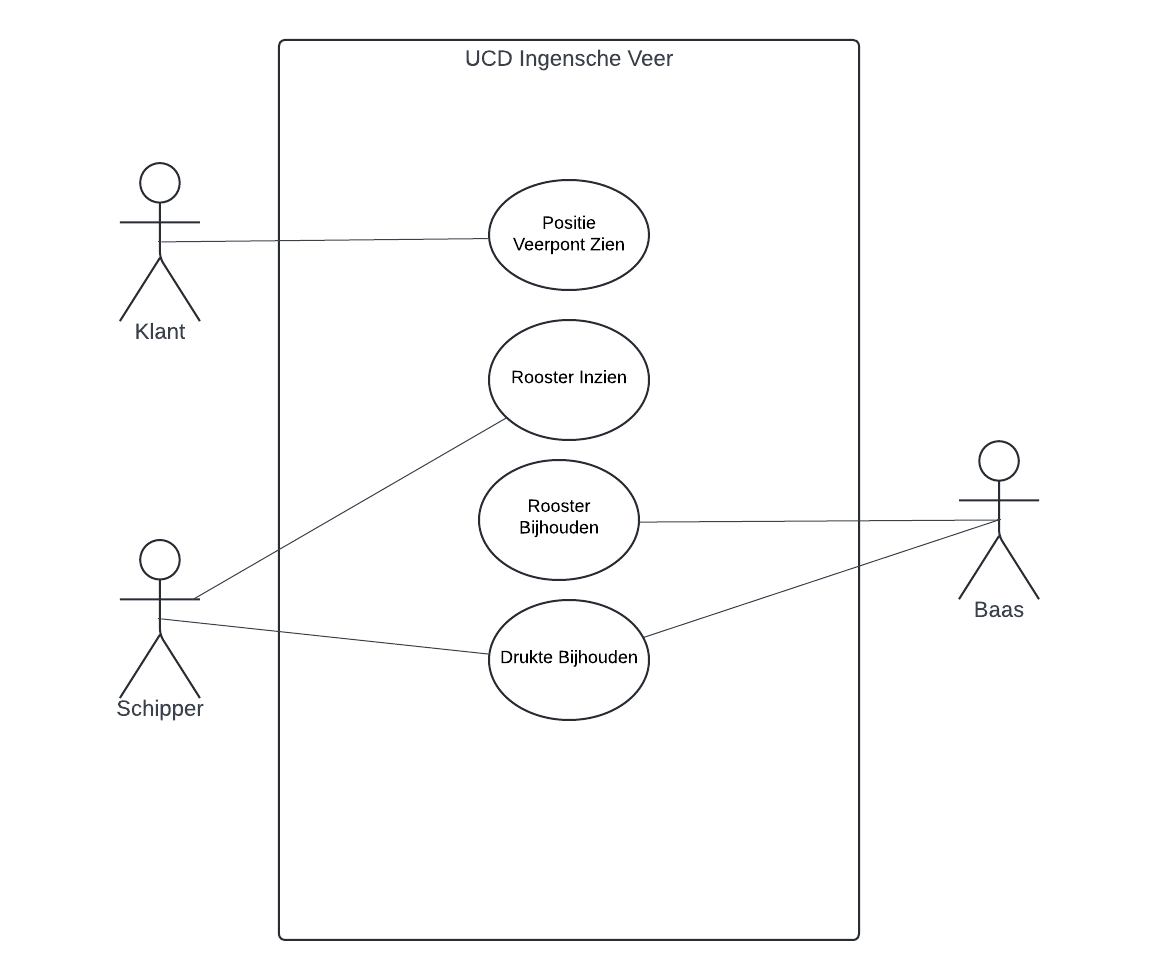
\includegraphics[width=0.7\textwidth]{images/iv_ucd.png}
    \caption{Use Case Diagram - Ingensche Veer}
\end{figure}

\subsection{Uitgangspunten, randvoorwaarden en aannames}
De belangrijkste punten aan het project zijn dat de data die wordt weergegeven klopt en dat de webapplicatie zelf betrouwbaar is. De applicatie moet dus niet zomaar crashen als er klanten op een bepaalde knop drukken.
Verder zijn er geen randvoorwaarden.

\section{Projectaanpak}
\subsection{Fase 1 - Plan van Aanpak}
De eerste fase heeft als doel het vaststellen van de aanpak van het project. Hiermee wordt het project concreet en wordt er een duidelijke planning opgesteld.  
Hieruit zal als resultaat een document voortkomen: het plan van aanpak. Dit document zal de basis vormen voor de rest van het project.
Deze fase zal een paar dagen duren en hier wil ik aan werken van 12-05-2024 tot 19-05-2024.
\subsubsection{Tools}
\begin{itemize}
    \item \textbf{Github} - Voor versiebeheer.
    \item \textbf{LaTeX} - Voor het schrijven van het PvA.
    \item \textbf{Vs Code} - Voor het schrijven van de tekst.
    \item \textbf{LucidChart} - Voor het maken van het use case diagram.
    \item \textbf{onlinegantt.com} - Voor het maken van de planning / gantt chart.
\end{itemize}


\subsection{Fase 2 - Sprint 1}
De tweede fase heeft als doel het ontwikkelen van de webapplicatie. Hierbij zal de focus liggen op het weergeven van de locatie van de veerpont en de algemene werking van de webapplicatie.
Het resultaat zal een werkende webapplicatie zijn die de locatie van de veerpont weergeeft, samen met de start van het ontwerpdocument.
Sprint 1 zal ongeveer twee weken duren, van 21 mei tot 4 juni.
\subsubsection{Tools}
\begin{itemize}
    \item \textbf{Java} - Voor het maken van de webapplicatie.
    \item \textbf{Aisstream.io} - Voor het ophalen van de locatie van de veerpont.
    \item \textbf{OpenStreetMap} - Voor het weergeven van de locatie van de veerpont.
    \item \textbf{VS Code} - Voor het schrijven van de code.
    \item \textbf{Github} - Voor versiebeheer.
\end{itemize}

\subsection{Fase 3 - Sprint 2}
De derde fase heeft als doel de overige use cases te implementeren, zoals het rooster en de drukte indicator. Ook zal de webapplicatie worden afgewerkt. 
Het resultaat zal de volledige webapplicatie zijn zoals hierboven beschreven. 
Sprint 2 zal duren van 7 juni tot 1 juli.
\subsubsection{Tools}
\begin{itemize}
    \item \textbf{Java} - Voor het maken van de webapplicatie.
    \item \textbf{Aisstream.io} - Voor het ophalen van de locatie van de veerpont.
    \item \textbf{OpenStreetMap} - Voor het weergeven van de locatie van de veerpont.
    \item \textbf{VS Code} - Voor het schrijven van de code.
    \item \textbf{Github} - Voor versiebeheer.
\end{itemize}

\subsection{Fase 4 - Poster}
De laatste fase is het maken van de poster voor de IPASS presentatie. Het resultaat hiervan zal een PDF zijn met hierop een poster die de samenvatting van het IPASS project representeert.
De poster maken zal ongeveer een dag duren. Dit wil ik in de laatste week van sprint 2 doen, zodat alles al goed uitgewerkt en duidelijk is.
\subsubsection{Tools}
\begin{itemize}
    \item \textbf{Canva} - Voor het maken van de poster.
\end{itemize}

\subsection{Planning}
De fases staan hierboven beschreven. De taken worden als onderverdeeld in sprints. De planning is te zien in de gantt chart in figuur 2.
\begin{figure}[h]
    \centering
    \label{fig:gc}
    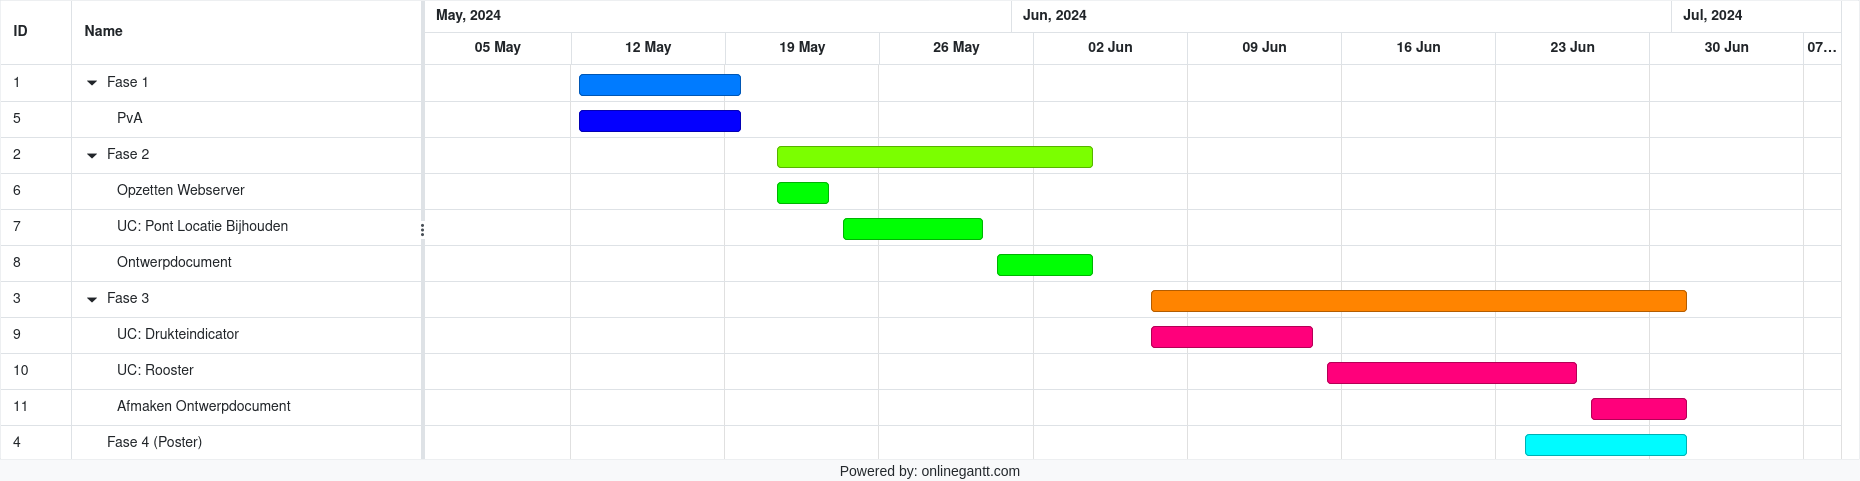
\includegraphics[width=1\textwidth]{images/gantt.png}
    \caption{Planning - Gantt chart}
\end{figure}


\section{Risico's}
% tabel
\subsection{Risico 1}
\begin{tcolorbox}[colback=white, colframe=orange, title=Risico 1]
\textbf{Risico:} Er wordt teveel tijd besteed aan opmaak, waardoor er minder tijd is voor andere onderdelen. \\
\textbf{Kans:} 3 \\
\textbf{Impact:} 8 \\
\textbf{Schade:} 24 \\
\textbf{Preventiemaatregel:} Per sprint wordt alleen aan de functionaliteit gewerkt. Zodra dit is afgerond, wordt de extra tijd besteed aan de opmaak. \\
\textbf{Oplossingsmaatregel:} Als er minder tijd is voor de opmaak, wordt er een simpele opmaak gemaakt. \\
\end{tcolorbox}

\subsection{Risico 2}
\begin{tcolorbox}[colback=white, colframe=red, title=Risico 2]
\textbf{Risico:} De AIS API wordt stopgezet. \\
\textbf{Kans:} 6 \\
\textbf{Impact:} 5 \\
\textbf{Schade:} 30 \\
\textbf{Preventiemaatregel:} Er wordt een betrouwbare API uitgekozen die al langer bestaat. \\
\textbf{Oplossingsmaatregel:} Als de API wegvalt, kan er een alternatief worden gekozen. AIS Data is immers in een universeel formaat. \\
\end{tcolorbox}

\subsection{Risico 3}
\begin{tcolorbox}[colback=white, colframe=green,coltitle=black, title=Risico 3 (Gehaald uit de template)]
\textbf{Risico:} De PC crasht met dataverlies\\
\textbf{Kans:} 3 \\
\textbf{Impact:} 7 \\
\textbf{Schade:} 21 \\
\textbf{Preventiemaatregel:} Er wordt regelmatig gebruik gemaakt van Github en er worden regelmatig back-ups gemaakt op externe harde schijven. \\
\textbf{Oplossingsmaatregel:} Alle data en code die op Github worden gepulld en de data op de externe harde schijven worden weer teruggezet op de nieuwe pc. \\
\end{tcolorbox}



\section{Referenties}
Er zijn geen referenties.


\end{document}